\documentclass[a4paper,10pt]{article}
\usepackage[utf8]{inputenc}
\usepackage{amsmath}
\usepackage{amsfonts}
\usepackage{amssymb}
\usepackage{algorithm}
\usepackage[noend]{algpseudocode}
\usepackage{program}
\usepackage{amsmath}
\usepackage{graphicx}
\usepackage[T1]{fontenc}
\usepackage{eso-pic}
\usepackage{gensymb}
\usepackage{listings}
\usepackage{float}
\lstloadlanguages{R}

\newcommand{\BackgroundPic}{\put(-4,0){\parbox[b][\paperheight]{\paperwidth}{\centering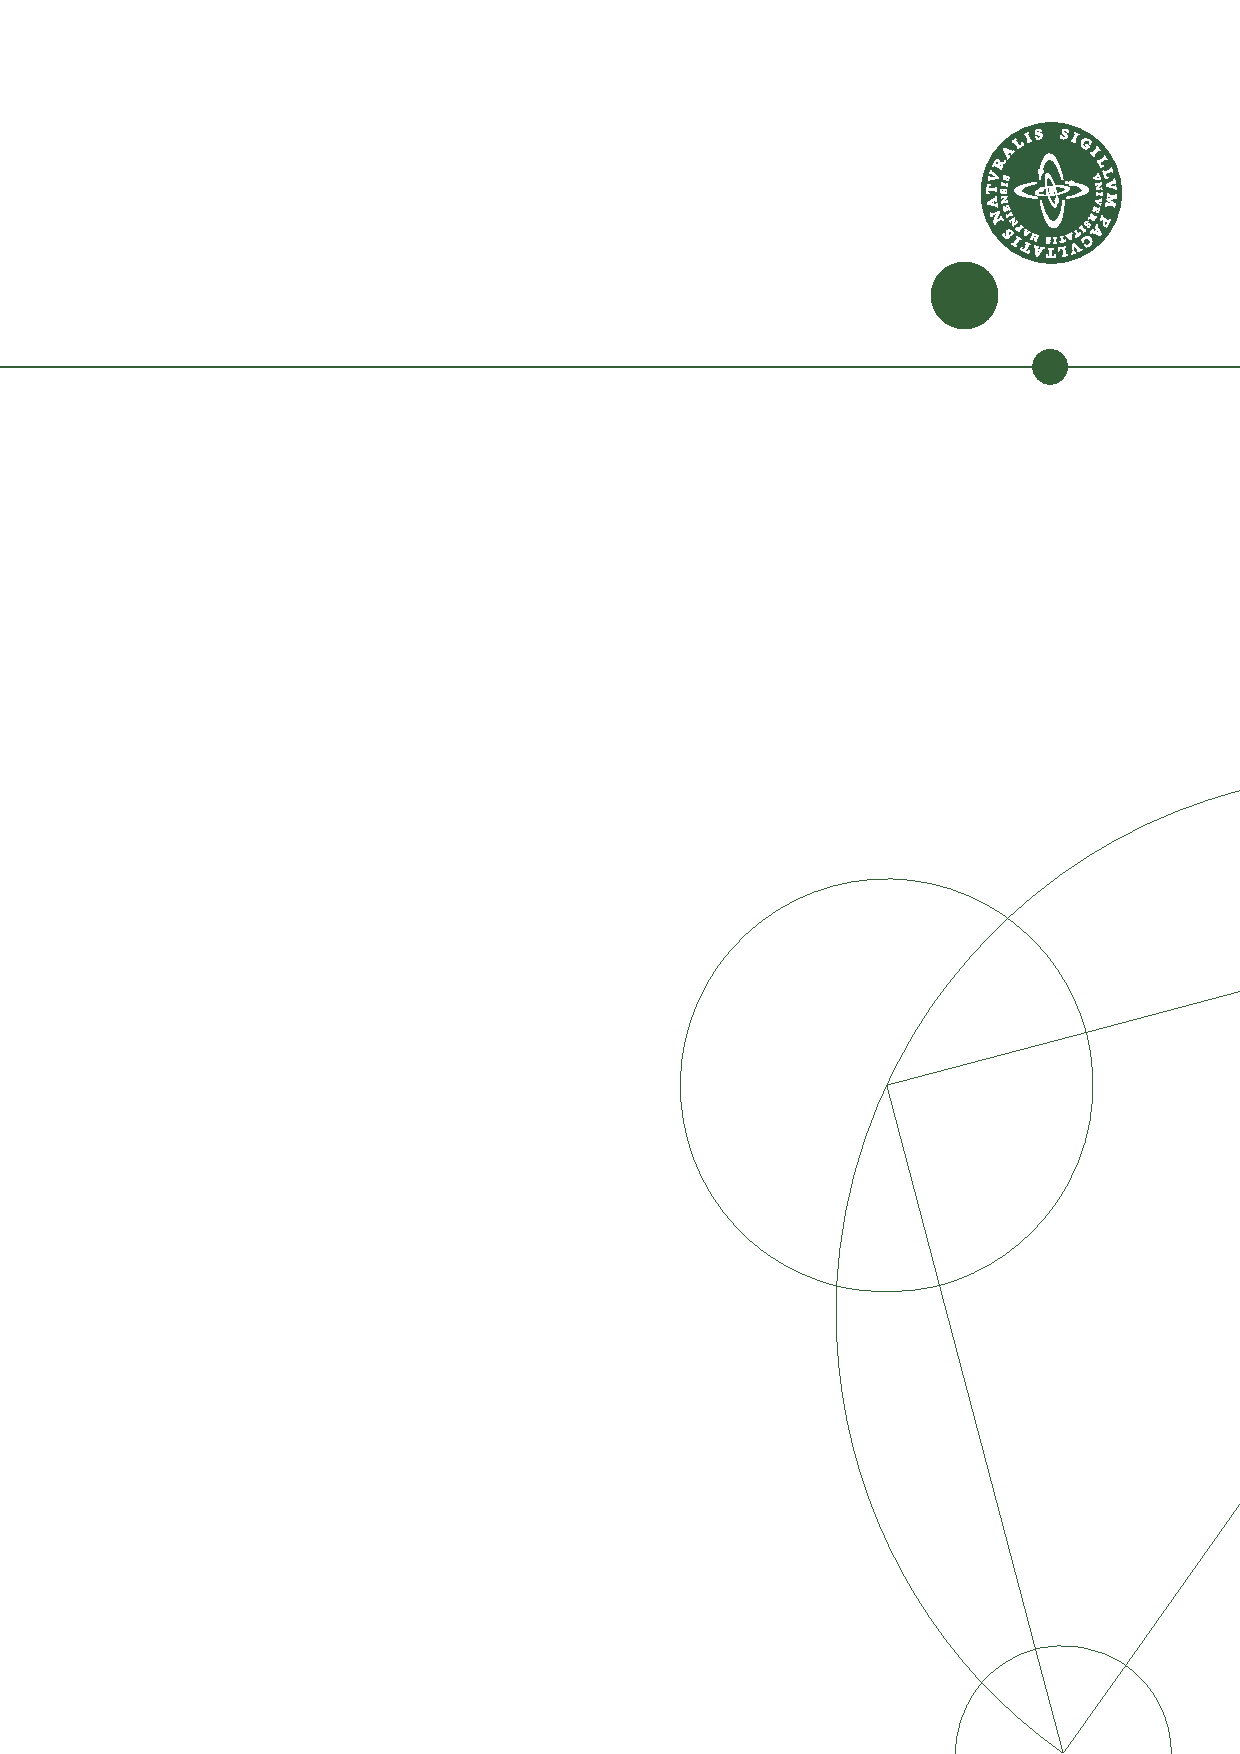
\includegraphics[width=\paperwidth,height=\paperheight]{nat-farve.pdf}}}}

\algnewcommand\True{\textbf{true}\space}
\algnewcommand\False{\textbf{false}\space}
\algdef{SE}[SUBALG]{Indent}{EndIndent}{}{\algorithmicend\ }%
\algtext*{Indent}
\algtext*{EndIndent}

\begin{document} 
	\AddToShipoutPicture*{\BackgroundPic}
	
	\begin{titlepage}
		\thispagestyle{empty}
		\vspace*{5cm}
		\begin{center}
			\Huge \textbf{Diskret Matematik og Algoritmer} \\
			\LARGE \textbf{Aflevering 8i} \\
		\end{center}
		\vspace*{3.5cm}
		\begin{flushleft}
			
		\begin{table}[h!]
			\begin{tabular}{lll}
				Adam Ingwersen,& \\ 
			\end{tabular}
		\end{table}
			
			
			\vspace{3mm}
			\vspace{3mm}
			Datalogisk  Institut\\
			Københavns Universitet\\
			\vspace{3mm}
			\today\\
			%\vspace*{0.5cm}
			
		\end{flushleft}
	\end{titlepage}

	\title{7g}
	\author{AAP}
	
	\newpage

\newpage

\section{}

\subsection{a)}
Her er det oplagt at illustrere relationen R via et relations-digraf. Dette er dog forholdsvist tidskrævende at skrive ind i LaTeX, hvorfor relationen vises som en liste, hhv. matrix. Relationen i matrix-format er umiddelbart en kopi af Tabel 1. 
\newline

\begin{figure}[H]
\centering
$R =$ \\
{(A,B),(B,A),(A,C),(C,A),(A,H),(H,A),\\
(B,C),(C,B),(B,D),(D,B),(B,F),(F,B),\\ 
(B,H),(H,B),(C,E),(E,C),(F,H),(H,F), \\
(G,I),(I,J),(J,G)}
\end{figure}

\begin{equation}
M_{R} = \begin{bmatrix}
        0 & 1 & 1 & 0 & 0 & 0 & 0 & 1 & 0 & 0 \\[0.3em]
        1 & 0 & 1 & 1 & 0 & 1 & 0 & 1 & 0 & 0 \\[0.3em]
        1 & 1 & 0 & 0 & 1 & 0 & 0 & 0 & 0 & 0 \\[0.3em]
        0 & 1 & 0 & 0 & 0 & 0 & 0 & 0 & 0 & 0 \\[0.3em]
        0 & 0 & 1 & 0 & 0 & 0 & 0 & 0 & 0 & 0 \\[0.3em]
        0 & 1 & 0 & 0 & 0 & 0 & 0 & 1 & 0 & 0 \\[0.3em]
        0 & 0 & 0 & 0 & 0 & 0 & 0 & 0 & 1 & 0 \\[0.3em]
        1 & 1 & 0 & 0 & 0 & 1 & 0 & 0 & 0 & 0 \\[0.3em]
        0 & 0 & 0 & 0 & 0 & 0 & 0 & 0 & 0 & 1 \\[0.3em]
        0 & 0 & 0 & 0 & 0 & 0 & 1 & 0 & 0 & 0 \\[0.3em]
\end{bmatrix}
\end{equation}

\subsection{b)}
Betragter $R^{\infty}$, som er den relation bestående af alle ordrede vetricer, der eksisterer - her inkluderes alle længder. Eftersom anse $R$ for at være delt op i to adskilte grupperinger, hvoraf den største gruppering er cyklisk i alle elementer; forventes det, at for at opskrive, $R^{\infty}$, skal der tilføjes alle alle relationer, der er længere end 1 til $R$:

\begin{figure}[H]
\centering
$R^{\infty} =$ \\
{(A,B),(B,A),(A,C),(C,A),(A,H),(H,A),\\
(B,C),(C,B),(B,D),(D,B),(B,F),(F,B),\\ 
(B,H),(H,B),(C,E),(E,C),(F,H),(H,F), \\
(G,I),(I,J),(J,G), \\
(A,E),(A,D,(A,F),(A,A),(B,E),(B,B),\\
(C,D),(C,F),(C,H),(C,C),(D,A),(D,C),\\
(D,D),(D,F),(D,H),(D,E),(E,B),(E,A),\\
(E,D),(E,F),(E,H),(E,E),(F,D),(F,C),\\
(F,E),(F,A),(F,F),(H,E),(H,C),(H,D),\\
(H,H),(G,J),(G,G),(I,G),(I,I),(J,I),(J,J)}
\end{figure}

\begin{equation}
M_{R^{\infty}} = \begin{bmatrix}
        1 & 1 & 1 & 1 & 1 & 1 & 0 & 1 & 0 & 0 \\[0.3em]
        1 & 1 & 1 & 1 & 1 & 1 & 0 & 1 & 0 & 0 \\[0.3em]
        1 & 1 & 1 & 1 & 1 & 1 & 0 & 1 & 0 & 0 \\[0.3em]
        1 & 1 & 1 & 1 & 1 & 1 & 0 & 1 & 0 & 0 \\[0.3em]
        1 & 1 & 1 & 1 & 1 & 1 & 0 & 1 & 0 & 0 \\[0.3em]
        1 & 1 & 1 & 1 & 1 & 1 & 0 & 1 & 0 & 0 \\[0.3em]
        0 & 0 & 0 & 0 & 0 & 0 & 1 & 0 & 1 & 1 \\[0.3em]
        1 & 1 & 1 & 1 & 1 & 1 & 0 & 1 & 0 & 0 \\[0.3em]
        0 & 0 & 0 & 0 & 0 & 0 & 1 & 0 & 1 & 1 \\[0.3em]
        0 & 0 & 0 & 0 & 0 & 0 & 1 & 0 & 1 & 1 \\[0.3em]
\end{bmatrix}
\end{equation}

\subsection{c)}



\end{document}